\section{}
A thin rectangular plate $a = \qty{30}{mm} \times b = \qty{15}{mm}$ is acted upon by a stress distribution 
(Fig. \ref{fig:Q1}) resulting in the uniform strain $\epsilon_x = \qty{400}{\mu}$, $\epsilon_y = \qty{200}{\mu}$,
and $\gamma_{xy} = \qty{-300}{\mu}$. Determine the changes in length of diagonals $\overline{QB}$ and $\overline{AC}$.
\begin{figure}[h]
    \centering
    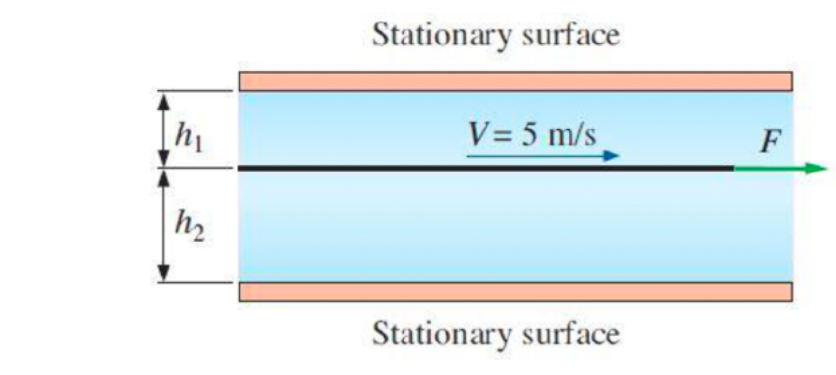
\includegraphics[width=0.5\linewidth]{Questions/Figures/Q1ProblemDiagram.png}
    \caption{Stress distribution on a thin rectangular plate.}
    \label{fig:Q1}
\end{figure}


First, the expression for the strain along $\overline{QB}$, $\epsilon_{x'}$, is governed by the following equation:
\begin{align}
    \epsilon_{x'} &= \epsilon_x\cos^2\theta + \epsilon_y\sin^2\theta + \gamma_{xy}\sin\theta\cos\theta \label{eq:Q1Strain}
\end{align}

The angle $\theta$ is given by:
\begin{align*}
    \theta &= \arctan\left(\frac{b}{a}\right) \\
    &= \arctan\left(\frac{15}{30}\right) \\
    &= \qty{26.57}{\degree}
\end{align*}

By the rectangular geometry,
\begin{align*}
    \phi = 180 - \theta &= \qty{153.4}{\degree}
\end{align*}

The length of the diagonals are given by:
\begin{align*}
    \overline{QB} = \overline{AC} &= \sqrt{a^2 + b^2} \\
    &= \sqrt{30^2 + 15^2} \\
    &= {\qty{33.54}{mm}}
\end{align*}

Using strain-displacement relations, the change in length of $\overline{QB}$ is given by:
\begin{align*}
    \Delta\overline{QB} &= \overline{QB}\epsilon_{x'} \\
    &= 33.54(400\times10^{-6}\cos^2(26.57) + 200\times10^{-6}\sin^2(26.57) - 300\times10^{-6}\sin(26.57)\cos(26.57)) \\
    &= \boxed{\qty{0.00805}{mm}}
\end{align*}

Similarly, $\Delta \overline{AC}$ is given by:
\begin{align*}
    \Delta\overline{AC} &= \overline{AC}\epsilon_{x'} \\
    &= 33.54(400\times10^{-6}\cos^2(153.4) + 200\times10^{-6}\sin^2(153.4) - 300\times10^{-6}\sin(153.4)\cos(153.4)) \\
    &= \boxed{\qty{0.0161}{mm}}
\end{align*}
